%----------------------------------------------------------------------------------------
%    PACKAGES AND THEMES
%----------------------------------------------------------------------------------------

\documentclass[aspectratio=169,xcolor=dvipsnames,9pt]{beamer}
\usetheme{SimpleDarkBlue}

\usepackage{hyperref}
\usepackage{graphicx}
\usepackage{booktabs}
\usepackage{amsmath}
\usepackage{amssymb}
\usepackage{tikz}
\usetikzlibrary{shapes.geometric, arrows.meta, positioning, calc, fit}
\usepackage{epstopdf}

%--- College logo on top-right corner of every slide ---
\addtobeamertemplate{frametitle}{}{%
    \begin{tikzpicture}[remember picture,overlay]
        \node[anchor=north east,yshift=2pt] at (current page.north east) {%
            
\includegraphics[height=0.8cm]{images/iiitm.eps}};
    \end{tikzpicture}
}

%--- Fix: override block templates to remove black title bars ---
\setbeamertemplate{block begin}{%
  \par\vskip\medskipamount%
  \begin{beamercolorbox}[colsep*=.75ex]{block title}%
    \usebeamerfont*{block title}\insertblocktitle%
  \end{beamercolorbox}%
  \nointerlineskip\vskip-0.5pt%
  \usebeamerfont{block body}%
  \begin{beamercolorbox}[colsep*=.75ex,vmode]{block body}%
    \vskip-.75ex\vbox{}%
}
\setbeamertemplate{block end}{%
  \end{beamercolorbox}\vskip\smallskipamount%
}
\setbeamertemplate{block alerted begin}{%
  \par\vskip\medskipamount%
  \begin{beamercolorbox}[colsep*=.75ex]{block title alerted}%
    \usebeamerfont*{block title alerted}\insertblocktitle%
  \end{beamercolorbox}%
  \nointerlineskip\vskip-0.5pt%
  \usebeamerfont{block body alerted}%
  \begin{beamercolorbox}[colsep*=.75ex,vmode]{block body alerted}%
    \vskip-.75ex\vbox{}%
}
\setbeamertemplate{block alerted end}{%
  \end{beamercolorbox}\vskip\smallskipamount%
}
\setbeamertemplate{block example begin}{%
  \par\vskip\medskipamount%
  \begin{beamercolorbox}[colsep*=.75ex]{block title example}%
    \usebeamerfont*{block title example}\insertblocktitle%
  \end{beamercolorbox}%
  \nointerlineskip\vskip-0.5pt%
  \usebeamerfont{block body example}%
  \begin{beamercolorbox}[colsep*=.75ex,vmode]{block body example}%
    \vskip-.75ex\vbox{}%
}
\setbeamertemplate{block example end}{%
  \end{beamercolorbox}\vskip\smallskipamount%
}

%----------------------------------------------------------------------------------------
%    TITLE PAGE
%----------------------------------------------------------------------------------------

\titlegraphic{
\includegraphics[height=1.4cm]{images/iiitm.eps}}

\title[Multi-Vehicle Detection]{Connected Component Analysis for\\Multi-Vehicle Detection in Shipment Tracking Systems}
\subtitle{B.Tech Project Presentation}

\author{Aditya Kumar Singh (2022IMG-005)}

\institute
{
    Under the supervision of \textbf{Prof.\ Kiran Kumar Pattanaik} \\[4pt]
    Department of Information Technology \\
    ABV Indian Institute of Information Technology and Management, Gwalior
}
\date{2026}

%----------------------------------------------------------------------------------------
%    PRESENTATION SLIDES
%----------------------------------------------------------------------------------------

\begin{document}

% ---- Slide 1: Title ----
\begin{frame}
    \titlepage
\end{frame}

% ---- Slide 2: Problem & Motivation ----
\begin{frame}{Problem \& Motivation}
    \begin{columns}[T]
        \column{0.55\textwidth}
        GPS-based shipment tracking generates \textbf{millions of records daily}. A critical data quality failure: a single shipment tracked by \textbf{multiple vehicles simultaneously}.

        \vspace{0.5em}
        \textbf{Root causes:} device misconfiguration, data integration errors, duplicate transmissions, system migration issues.

        \vspace{0.5em}
        \textbf{Observable symptoms:}
        \begin{itemize}
            \item \textbf{Impossible teleportation} --- Shanghai to Shenzhen (1{,}200 km) in 5 min
            \item \textbf{Oscillating locations} --- jumping between distant areas
            \item \textbf{Concurrent distant positions}
        \end{itemize}

        \column{0.42\textwidth}
        \begin{alertblock}{Business Impact}
            \begin{itemize}
                \item Customer confusion
                \item Incorrect ETAs
                \item Billing disputes
                \item Operational blindness
                \item SLA violations
            \end{itemize}
        \end{alertblock}

        \vspace{0.3em}
        \begin{block}{Challenge}
            Must distinguish errors from \textbf{legitimate handovers} (e.g.\ truck $\to$ ship at port).
        \end{block}
    \end{columns}
\end{frame}

% ---- Slide 3: Real-World Illustrations ----
\begin{frame}{The Problem in Practice}
    \begin{columns}[c]
        \column{0.48\textwidth}
        \centering
        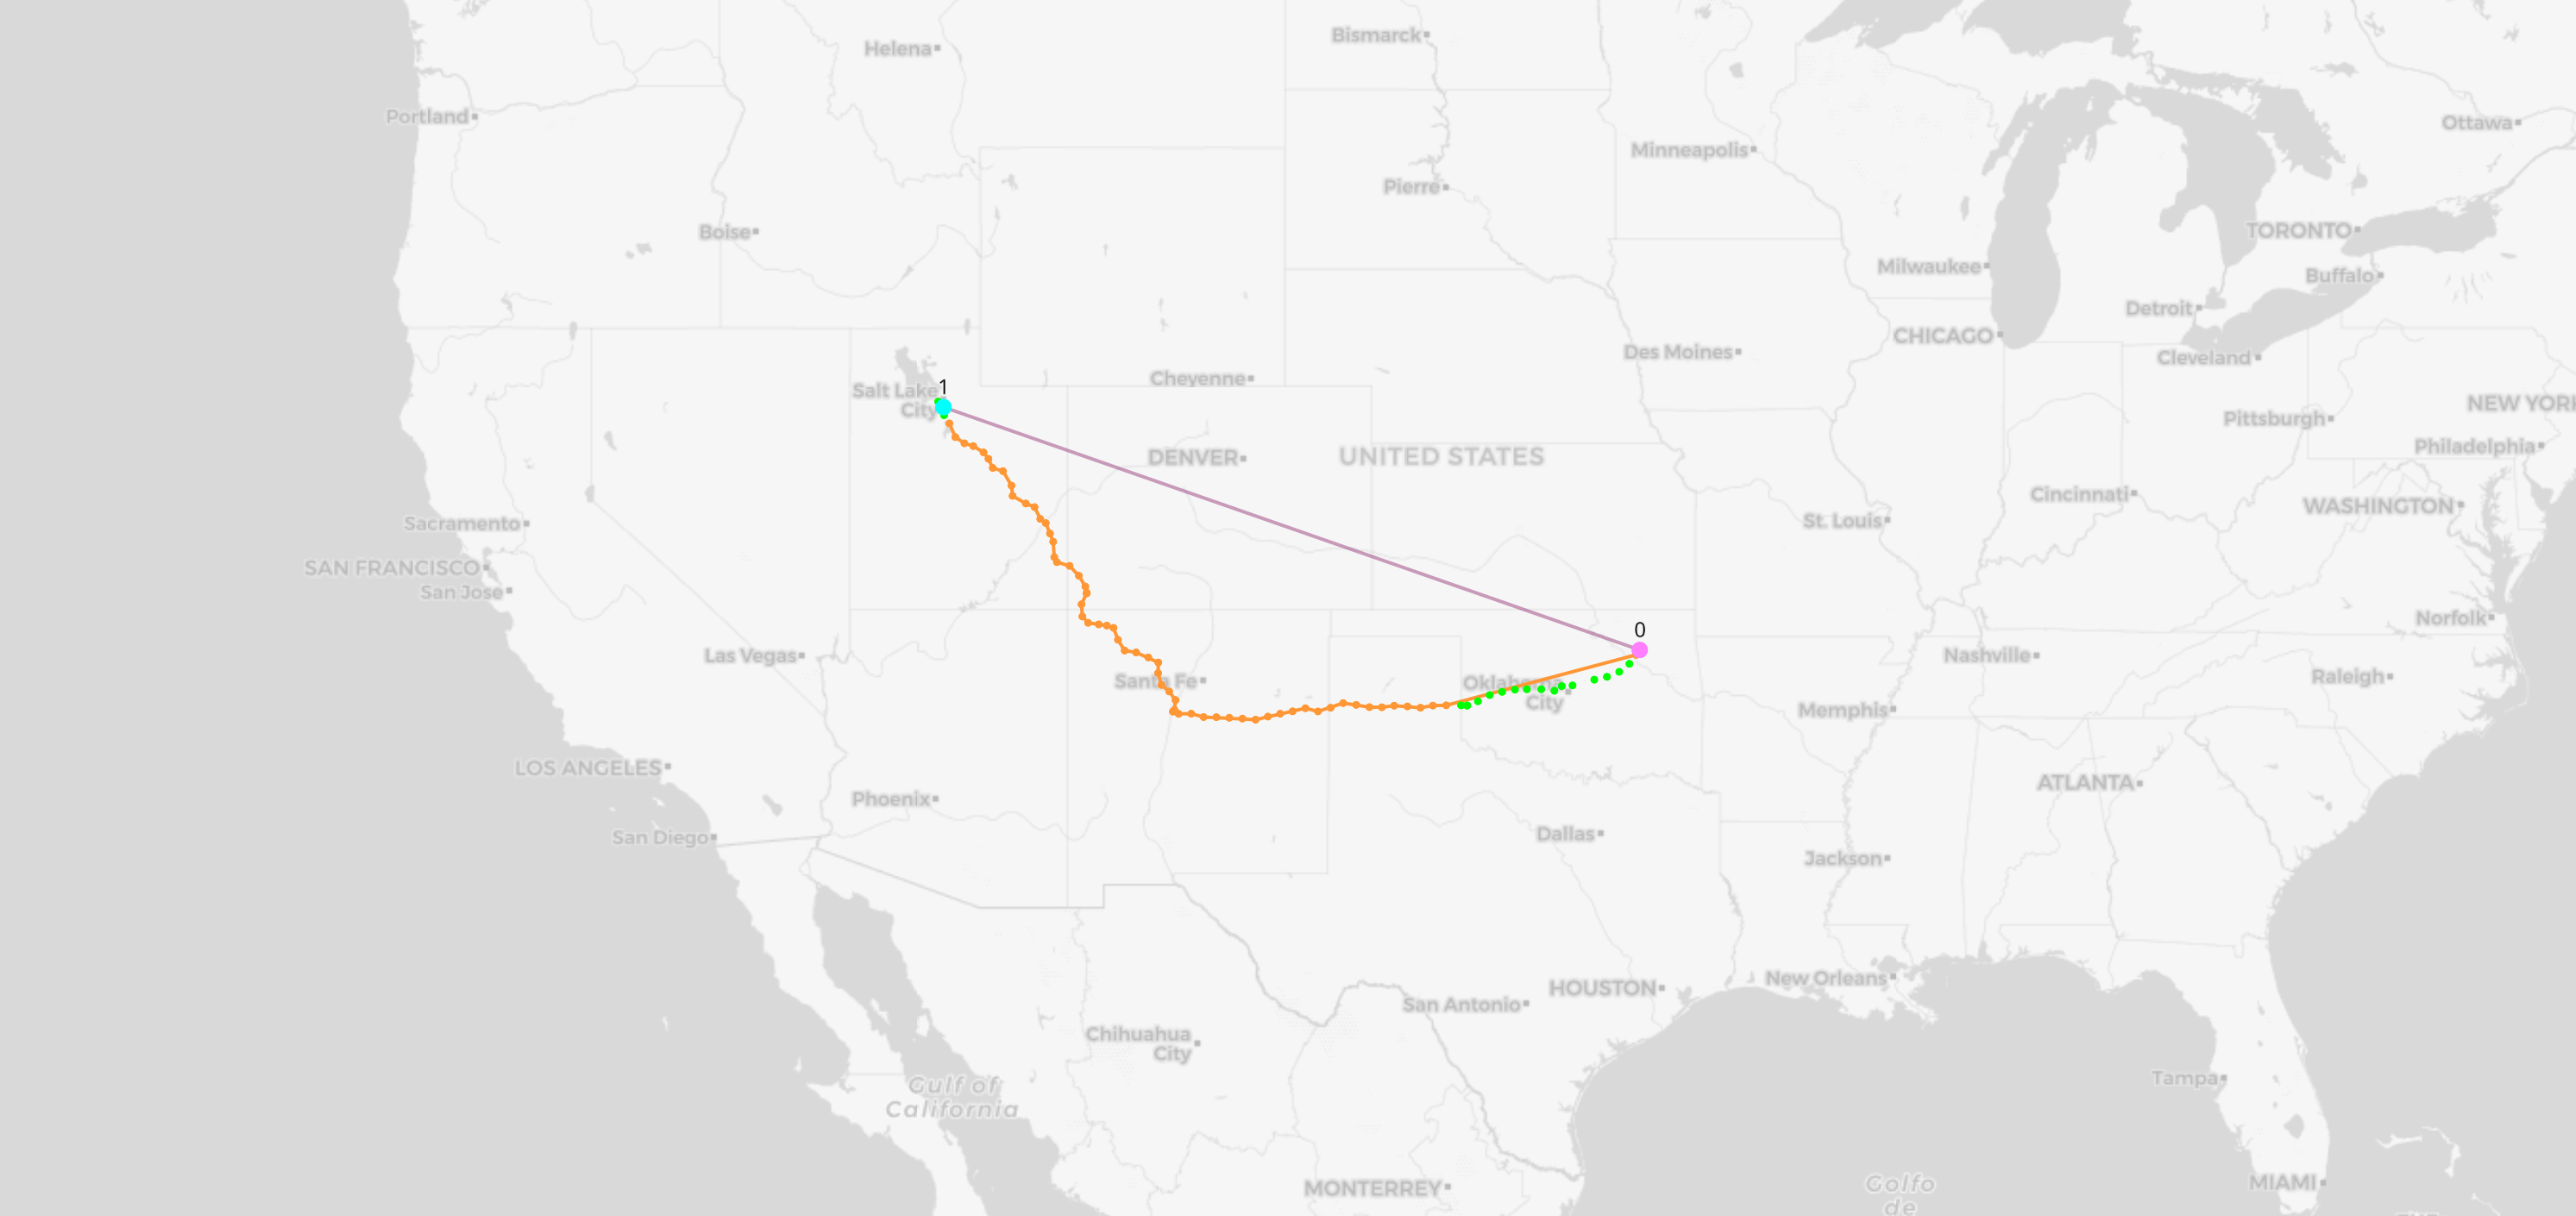
\includegraphics[width=0.85\linewidth,height=0.3\textheight,keepaspectratio]{images/Shipment-tracking.png}\\[0.2em]
        {\scriptsize A typical GPS-based shipment tracking interface}

        \column{0.48\textwidth}
        \centering
        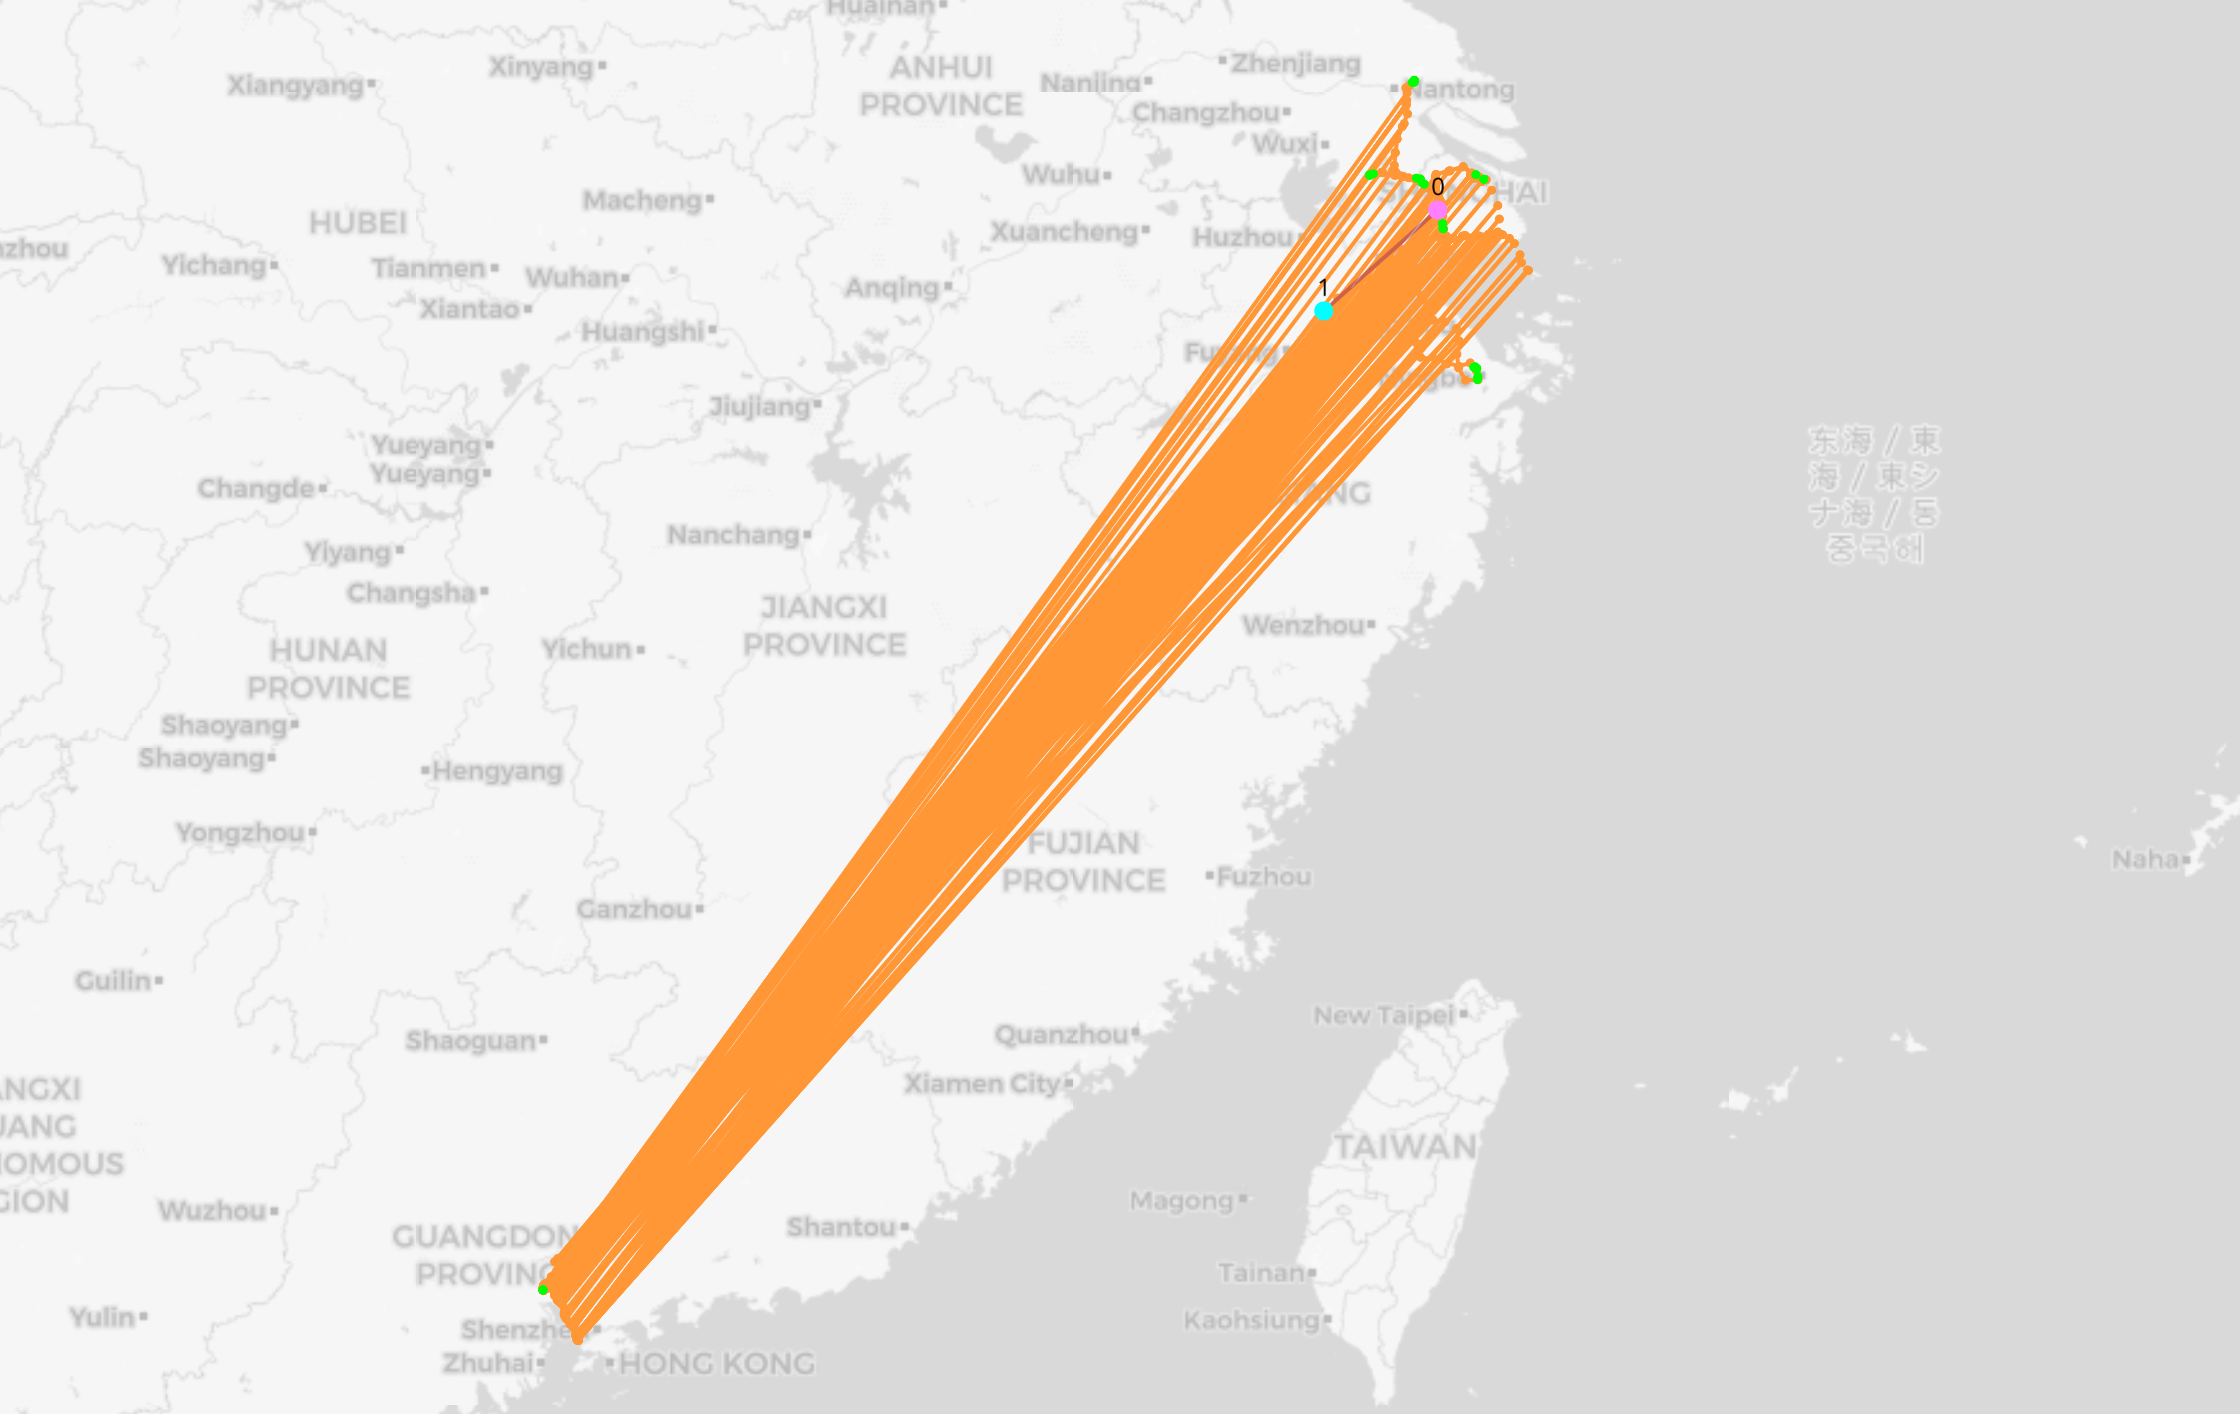
\includegraphics[width=0.85\linewidth,height=0.3\textheight,keepaspectratio]{images/multiple-vehicles-before.png}\\[0.2em]
        {\scriptsize \textcolor{red}{Before:} Conflicting GPS trails from two devices}
    \end{columns}

    \vspace{0.3em}

    \begin{columns}[c]
        \column{0.48\textwidth}
        \centering
        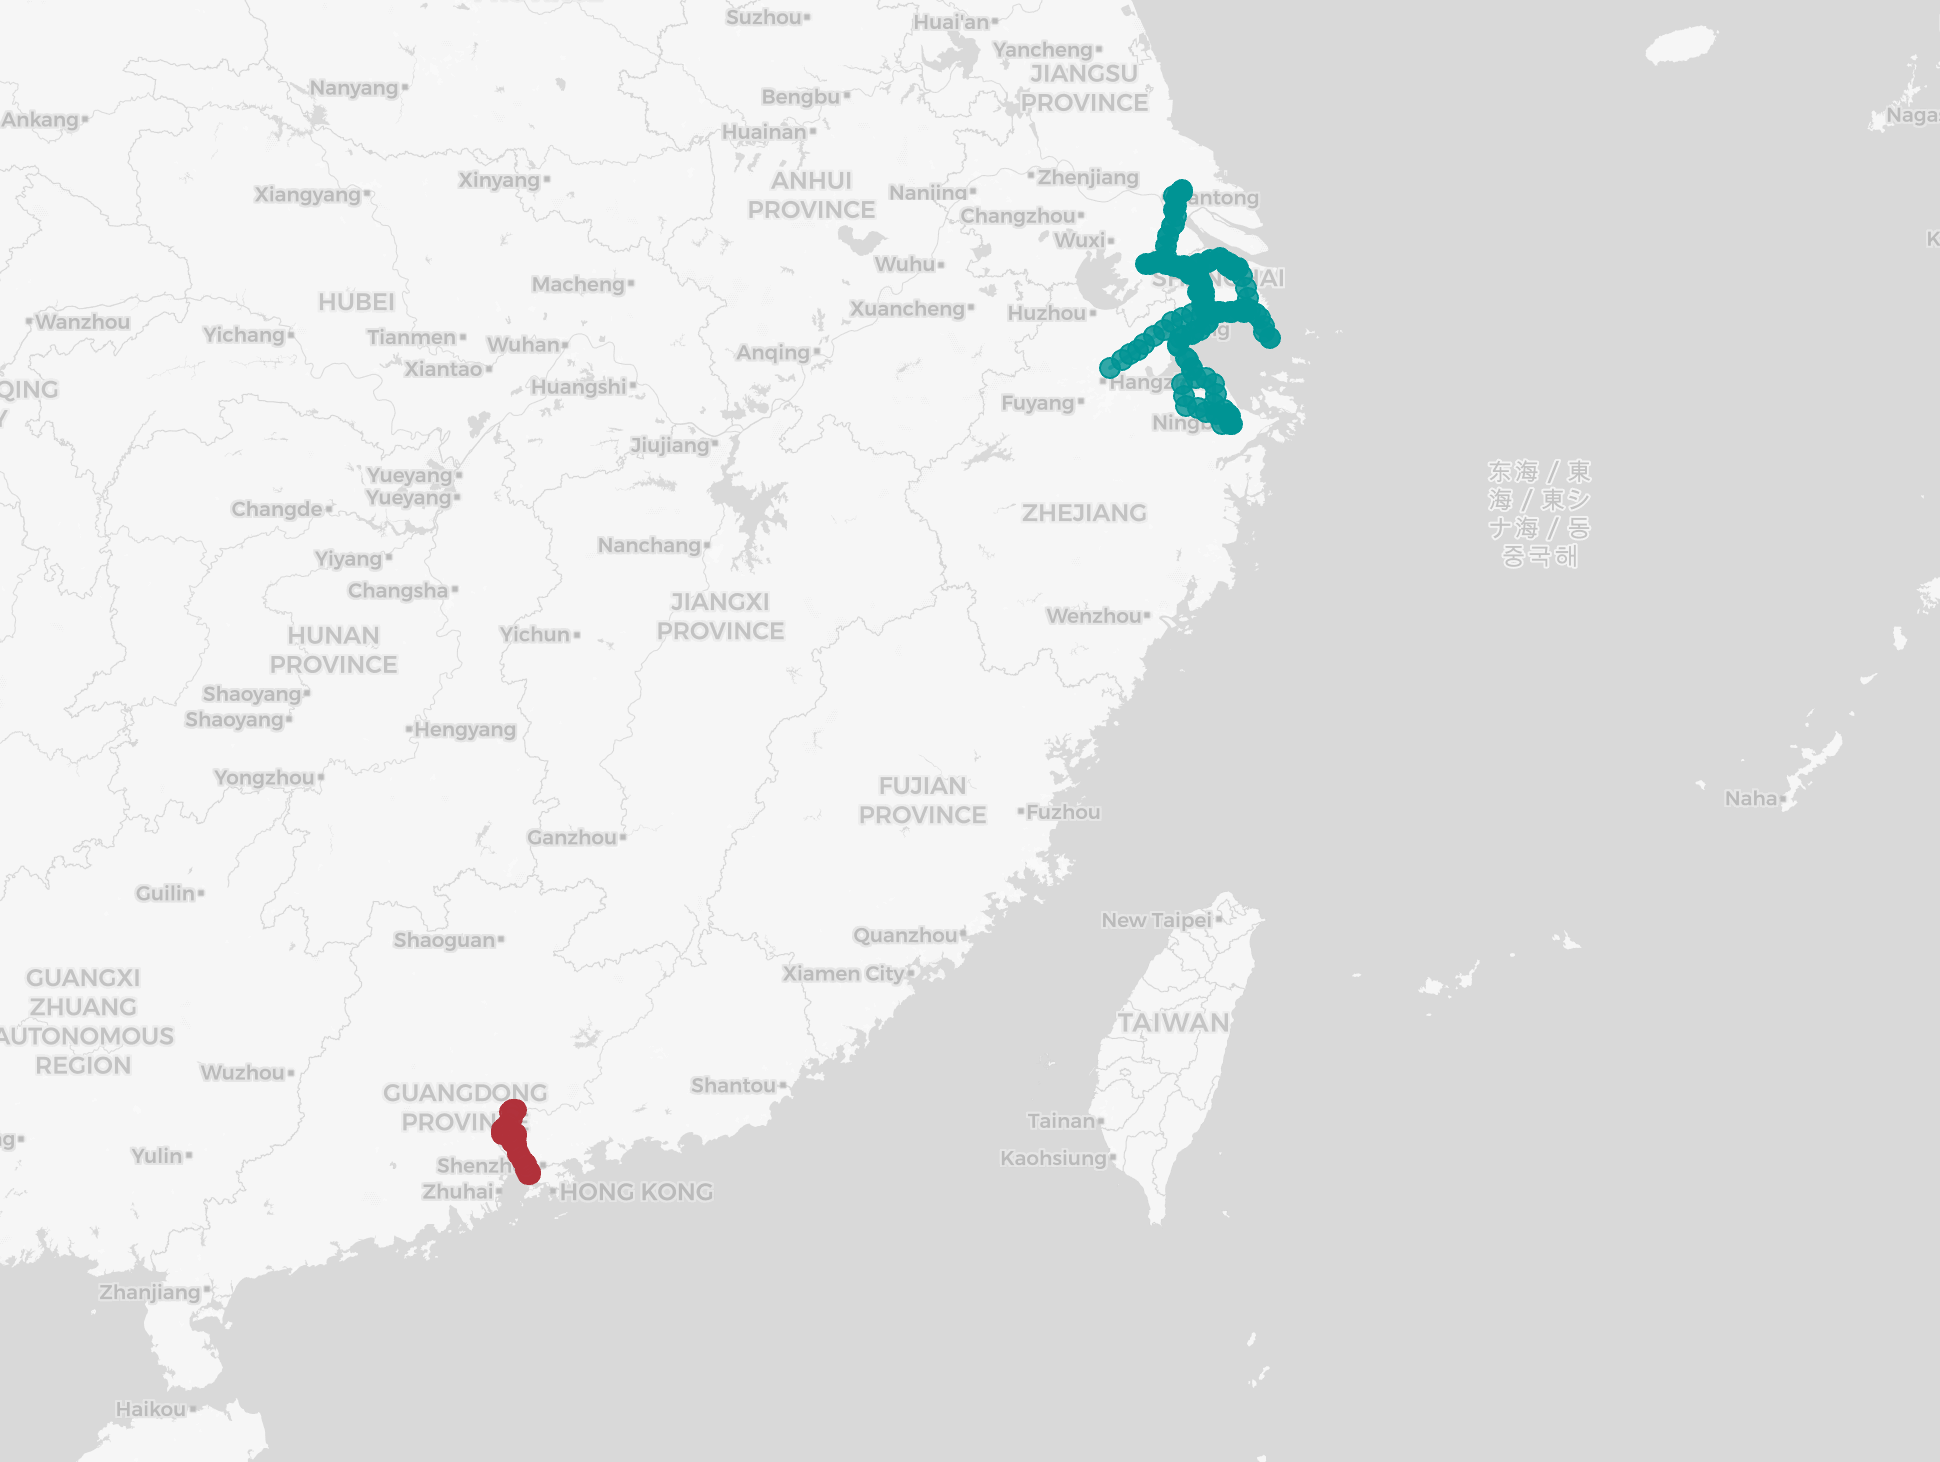
\includegraphics[width=0.85\linewidth,height=0.3\textheight,keepaspectratio]{images/multiple-vehicles after.png}\\[0.2em]
        {\scriptsize \textcolor{green!50!black}{After:} Trails separated, anomaly identified}

        \column{0.48\textwidth}
        \centering
        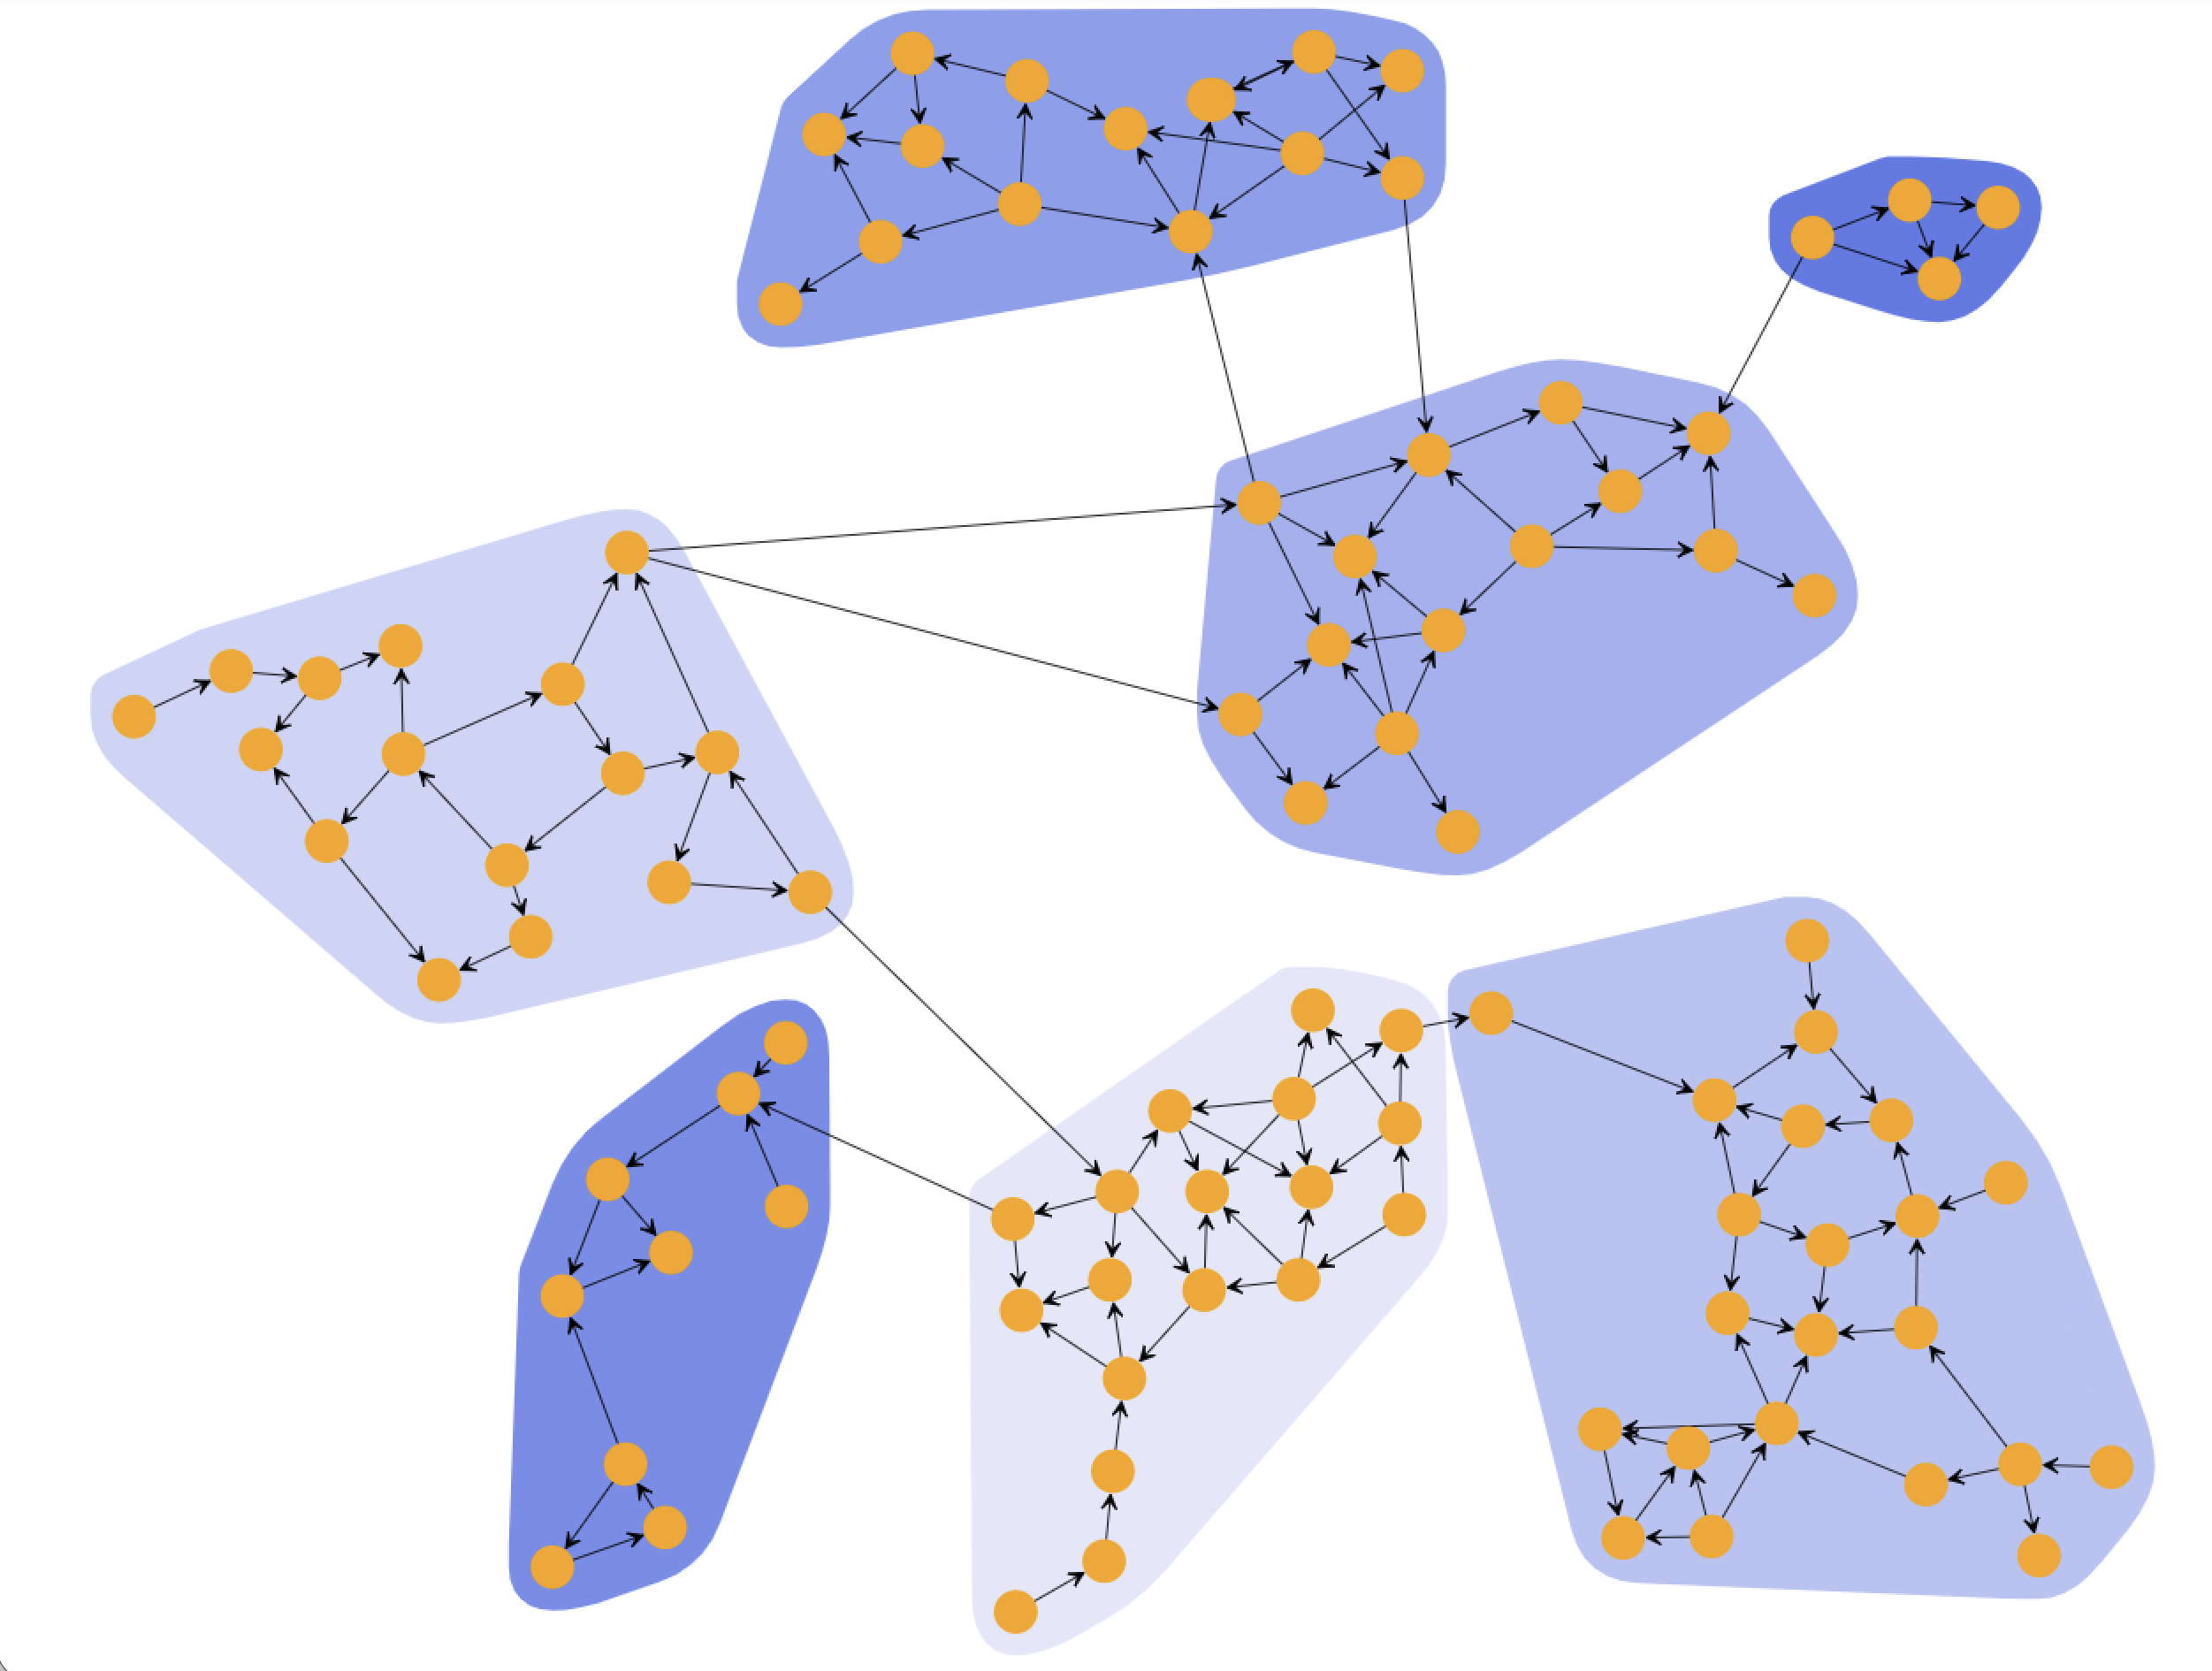
\includegraphics[width=0.85\linewidth,height=0.3\textheight,keepaspectratio]{images/graph-clustering-edege-colored-segregation.png}\\[0.2em]
        {\scriptsize Connected components color-coded by cluster}
    \end{columns}
\end{frame}

% ---- Slide 4: System Overview ----
\begin{frame}{Proposed Framework: System Overview}
    \centering
    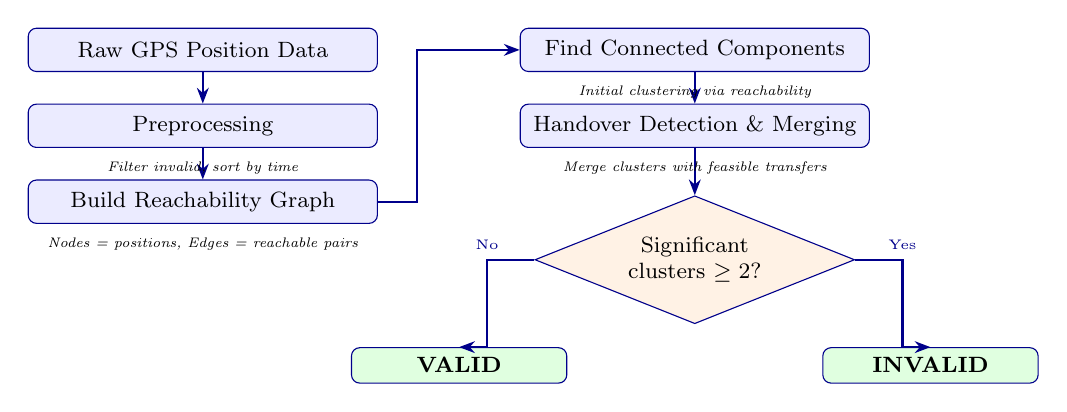
\begin{tikzpicture}[
        node distance=0.4cm and 1.2cm,
        block/.style={rectangle, draw=DarkBlue, fill=blue!8, text width=4.2cm, minimum height=0.55cm, align=center, rounded corners=3pt, font=\footnotesize},
        decision/.style={diamond, draw=DarkBlue, fill=orange!10, text width=1.8cm, minimum height=0.5cm, align=center, aspect=2.5, font=\footnotesize},
        io/.style={rectangle, draw=DarkBlue, fill=green!12, text width=2.5cm, minimum height=0.45cm, align=center, rounded corners=3pt, font=\footnotesize\bfseries},
        arrow/.style={-{Stealth[length=2mm]}, thick, DarkBlue},
    ]
        % Left column
        \node[block] (input) {Raw GPS Position Data};
        \node[block, below=of input] (preprocess) {Preprocessing};
        \node[block, below=of preprocess] (graph) {Build Reachability Graph};

        % Right column
        \node[block, right=1.8cm of input] (cluster) {Find Connected Components};
        \node[block, below=of cluster] (handover) {Handover Detection \& Merging};
        \node[decision, below=0.6cm of handover] (decide) {Significant clusters $\geq 2$?};

        % Results
        \node[io, below left=0.7cm and 0.6cm of decide] (valid) {VALID};
        \node[io, below right=0.7cm and 0.6cm of decide] (invalid) {INVALID};

        % Arrows: left column down
        \draw[arrow] (input) -- (preprocess);
        \draw[arrow] (preprocess) -- (graph);

        % Arrow: left to right
        \draw[arrow] (graph.east) -- ++(0.5,0) |- (cluster.west);

        % Arrows: right column down
        \draw[arrow] (cluster) -- (handover);
        \draw[arrow] (handover) -- (decide);

        % Decision arrows
        \draw[arrow] (decide.west) -- ++(-0.6,0) node[above, font=\tiny] {No} |- (valid.north);
        \draw[arrow] (decide.east) -- ++(0.6,0) node[above, font=\tiny] {Yes} |- (invalid.north);

        % Labels
        \node[font=\tiny\itshape, below=0.05cm of preprocess] {Filter invalid, sort by time};
        \node[font=\tiny\itshape, below=0.05cm of graph] {Nodes = positions, Edges = reachable pairs};
        \node[font=\tiny\itshape, below=0.05cm of cluster] {Initial clustering via reachability};
        \node[font=\tiny\itshape, below=0.05cm of handover] {Merge clusters with feasible transfers};
    \end{tikzpicture}
\end{frame}

% ---- Slide 4: Graph Theory Background ----
\begin{frame}{Graph Theory Background}
    \begin{columns}[T]
        \column{0.48\textwidth}
        \begin{block}{Fundamental Definitions}
            \begin{itemize}
                \item \textbf{Graph} $G = (V, E)$: vertices + edges
                \item \textbf{Directed graph}: edge $(u,v) \neq (v,u)$
                \item \textbf{DAG}: directed, no cycles
                \item \textbf{Connected component}: maximal subgraph where every pair is connected
            \end{itemize}
        \end{block}

        \begin{block}{Haversine Distance}
            \small
            \[
            d = 2R \cdot \arcsin\!\!\sqrt{\sin^2\!\frac{\Delta\phi}{2} + \cos\phi_i\cos\phi_j\sin^2\!\frac{\Delta\lambda}{2}}
            \]
            $R = 6{,}371$ km. Error $< 0.3\%$ vs.\ ellipsoidal.
        \end{block}

        \column{0.48\textwidth}
        \begin{block}{Notation}
            \small
            \begin{tabular}{ll}
                $p_i = (\text{lat}, \text{lon}, t)$ & Position \\
                $P = \{p_1, \ldots, p_n\}$ & Sorted sequence \\
                $V_{\max} = 69.4$ m/s & Max speed \\
                $\tau = 1800$ s & Jitter window \\
                $T_H = 28800$ s & Handover window \\
                $\alpha = 0.10$ & Min cluster \% \\
                $s_{\min} = 5$ & Min cluster size \\
            \end{tabular}
        \end{block}

        \begin{block}{Reachability}
            $p_2$ reachable from $p_1$ iff:
            \[
            d(p_1, p_2) \leq V_{\max} \cdot (t_2 - t_1)
            \]
        \end{block}
    \end{columns}
\end{frame}

% ---- Slide 5: Graph Formulation ----
\begin{frame}{Graph Formulation}
    \begin{block}{Position Reachability Graph $G = (V, E)$}
        \begin{itemize}
            \item Each GPS position $p_i = (\text{lat}, \text{lon}, t)$ is a \textbf{vertex}
            \item Edge $(p_i, p_j)$ exists iff movement is physically feasible:
        \end{itemize}
        \[
        \mathrm{reachable}(p_i, p_j) \iff \underbrace{d(p_i, p_j)}_{\text{Haversine}} \leq V_{\max} \cdot (t_j - t_i), \qquad V_{\max} = 250 \text{ km/h}
        \]
    \end{block}

    \vspace{0.3em}

    \begin{columns}[T]
        \column{0.48\textwidth}
        \begin{block}{Jitter Tolerance}
            GPS noise handled by checking \textbf{multiple recent} positions within $\tau = 30$ min window:
            \[
            \exists\, p_i \in W(p_j, C, \tau) : \mathrm{reachable}(p_i, p_j)
            \]
        \end{block}

        \column{0.48\textwidth}
        \begin{block}{Handover Detection}
            Legitimate transfers (truck $\to$ ship) detected via boundary positions of adjacent clusters:
            \[
            |t_i - t_j| \leq 8\text{h} \;\wedge\; \mathrm{reachable}(p_i, p_j)
            \]
        \end{block}
    \end{columns}
\end{frame}

% ---- Slide 5: Key Theorems ----
\begin{frame}{Key Theorems \& Properties}
    \begin{block}{Theorem 1: Single Component $\Rightarrow$ Single Vehicle}
        If the Position Reachability Graph has exactly one weakly connected component, all positions are consistent with single-vehicle tracking.
    \end{block}

    \vspace{0.3em}

    \begin{alertblock}{Theorem 2: Multiple Large Components $\Rightarrow$ Multiple Vehicles}
        If $G$ has $\geq 2$ components each containing $\geq 10\%$ of total positions, multiple vehicles are tracking the shipment.
    \end{alertblock}

    \vspace{0.3em}

    \begin{block}{Theorem 3: Handover Preserves Validity}
        If two components can be merged via a valid handover, the merged component represents valid single-vehicle tracking (with transfer).
    \end{block}

    \vspace{0.3em}

    \textbf{Graph properties:} always a DAG (edges follow time), reachability is \textbf{non-transitive}, significance filters noise: $\mathrm{significant}(C) \iff |C| \geq \max(5,\; 0.10 \cdot n)$
\end{frame}

% ---- Slide 6: Algorithm Design ----
\begin{frame}{Algorithm: SingleVehicleCheck}
    \begin{columns}[T]
        \column{0.52\textwidth}
        \centering
        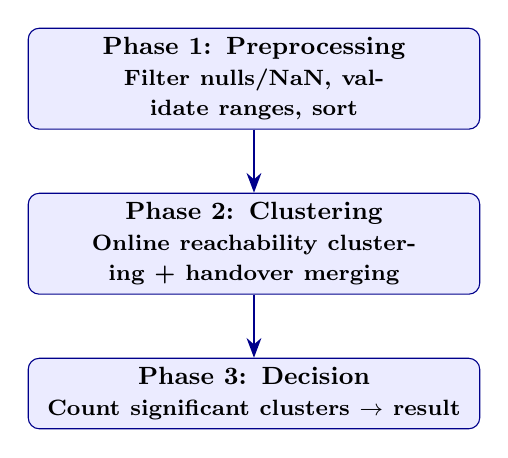
\begin{tikzpicture}[
            phase/.style={rectangle, draw=DarkBlue, fill=blue!8, text width=5.5cm, minimum height=0.7cm, align=center, rounded corners=4pt, font=\small\bfseries},
            arrow/.style={-{Stealth[length=2.5mm]}, thick, DarkBlue}
        ]
            \node[phase] (p1) {Phase 1: Preprocessing \\ {\footnotesize Filter nulls/NaN, validate ranges, sort}};
            \node[phase, below=0.8cm of p1] (p2) {Phase 2: Clustering \\ {\footnotesize Online reachability clustering + handover merging}};
            \node[phase, below=0.8cm of p2] (p3) {Phase 3: Decision \\ {\footnotesize Count significant clusters $\to$ result}};
            \draw[arrow] (p1) -- (p2);
            \draw[arrow] (p2) -- (p3);
        \end{tikzpicture}

        \column{0.45\textwidth}
        \begin{block}{Clustering (Phase 2)}
            For each position chronologically:
            \begin{enumerate}
                \item Check recent positions in existing clusters (jitter window $\tau$, up to 3)
                \item \textbf{Reachable?} $\to$ assign to cluster
                \item \textbf{Not?} $\to$ new cluster
            \end{enumerate}
            Then merge clusters via handover predicate.
        \end{block}

        \begin{block}{Decision (Phase 3)}
            0 significant $\to$ UNCERTAIN\\
            1 significant $\to$ TRUE\\
            $\geq 2$ significant $\to$ \alert{FALSE}
        \end{block}
    \end{columns}
\end{frame}

% ---- Slide 7: Worked Example ----
\begin{frame}{Worked Example: Shanghai \& Shenzhen}
    \begin{columns}[T]
        \column{0.52\textwidth}
        \begin{block}{Input (6 GPS positions)}
            \footnotesize
            \begin{tabular}{llll}
                $p_1$: & Shanghai & 31.23\textdegree N & 08:00 \\
                $p_2$: & Shenzhen & 22.55\textdegree N & 08:15 \\
                $p_3$: & Shanghai & 31.24\textdegree N & 09:00 \\
                $p_4$: & \textcolor{red}{NaN} & & 09:30 \\
                $p_5$: & Shenzhen & 22.56\textdegree N & 10:00 \\
                $p_6$: & Shanghai & 31.25\textdegree N & 10:30 \\
            \end{tabular}
        \end{block}

        \textbf{Preprocess:} remove $p_4$ $\to$ 5 valid positions.

        \textbf{Cluster:} Shanghai $\{p_1, p_3, p_6\}$, Shenzhen $\{p_2, p_5\}$. No cross-edges (1{,}200 km in 15 min = impossible).

        \column{0.45\textwidth}
        \begin{block}{Connected Components}
            \centering
            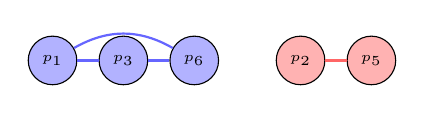
\begin{tikzpicture}[>=Stealth, scale=0.9]
                \node[circle, draw, fill=blue!30, minimum size=0.5cm, font=\tiny\bfseries] (p1) at (0,0) {$p_1$};
                \node[circle, draw, fill=blue!30, minimum size=0.5cm, font=\tiny\bfseries] (p3) at (1,0) {$p_3$};
                \node[circle, draw, fill=blue!30, minimum size=0.5cm, font=\tiny\bfseries] (p6) at (2,0) {$p_6$};
                \draw[blue!60, thick] (p1) -- (p3);
                \draw[blue!60, thick] (p3) -- (p6);
                \draw[blue!60, thick, bend left=30] (p1) to (p6);
                \node[circle, draw, fill=red!30, minimum size=0.5cm, font=\tiny\bfseries] (p2) at (3.5,0) {$p_2$};
                \node[circle, draw, fill=red!30, minimum size=0.5cm, font=\tiny\bfseries] (p5) at (4.5,0) {$p_5$};
                \draw[red!60, thick] (p2) -- (p5);
            \end{tikzpicture}
        \end{block}

        \vspace{0.3em}

        \begin{alertblock}{Decision}
            $n = 5$, threshold $= \max(5, 0.5) = 5$\\
            Significant clusters $= 2$\\[0.3em]
            \textbf{Result: FALSE}\\
            Multiple vehicles detected.
        \end{alertblock}
    \end{columns}
\end{frame}

% ---- Slide 8: Complexity ----
\begin{frame}{Complexity Analysis \& Edge Cases}
    \begin{columns}[T]
        \column{0.52\textwidth}
        \begin{table}
            \centering
            \begin{tabular}{lcc}
                \toprule
                \textbf{Phase} & \textbf{Time} & \textbf{Space} \\
                \midrule
                Preprocessing & $O(n \log n)$ & $O(n)$ \\
                Clustering & $O(n \cdot m)$ & $O(n)$ \\
                Handover Merge & $O(m^3 \cdot b^2)$ & $O(m)$ \\
                Decision & $O(m)$ & $O(1)$ \\
                \midrule
                \textbf{Total} & $O(n \log n + m^3 b^2)$ & $O(n)$ \\
                \bottomrule
            \end{tabular}
        \end{table}

        \vspace{0.3em}
        $n$ = positions, $m$ = clusters ($m \ll n$), $b = 5$.\\
        Typical case ($m < 10$): effectively \textbf{$O(n \log n)$}.

        \column{0.45\textwidth}
        \begin{block}{Edge Case Handling}
            \begin{table}
                \centering
                \small
                \begin{tabular}{ll}
                    \toprule
                    \textbf{Case} & \textbf{Result} \\
                    \midrule
                    No positions & UNCERTAIN \\
                    Single position & TRUE \\
                    All invalid & UNCERTAIN \\
                    $\Delta t = 0$ & 100 m tolerance \\
                    \bottomrule
                \end{tabular}
            \end{table}
        \end{block}

        \vspace{0.3em}

        \begin{block}{Input Validation}
            Null, NaN, and range checks on coordinates and timestamps before processing.
        \end{block}
    \end{columns}
\end{frame}

% ---- Slide 10: Thank You ----
\begin{frame}
    \Huge{\centerline{\textbf{Thank You}}}
    \vspace{1em}
    \normalsize{\centerline{Questions?}}
\end{frame}

%----------------------------------------------------------------------------------------

\end{document}
